
\documentclass[a4paper, 12pt, reqno]{amsart}

\usepackage[T1]{fontenc}
\usepackage[margin=3cm]{geometry}
\usepackage[parfill]{parskip} %Spaces for paragraphs

%Line spacing
\usepackage{setspace}
\setstretch{1.25}

\usepackage{verbatim}
\usepackage{dsfont} %Double stroke font
\usepackage{amsmath}
\usepackage{natbib}
\usepackage{graphicx}

%For adding spacing before section titles
\newcommand{\ssection}[1]{\vspace{1cm}\section{#1}}
\newcommand{\ssubsection}[1]{\vspace{0.25cm}\subsection{#1}}

%Defining an environment for examples
\newcounter{mathexample}[section]
\newenvironment{mathexample}
{
	\refstepcounter{mathexample} %Increment environment counter
	\textbf{Example \themathexample} 
	\\
}
{
	\vspace{1cm}
}

\title{USRA 2022 Recap}
\author{Zach Strong}
\date{\today}

\begin{document}
	\maketitle
	\tableofcontents
	
	\ssection{Explanation}
		This LaTeX file was created to explain some of the most important aspects of my 2022 summer 
		research funded by NSERC's USRA. Its intention is to serve as a guide for where to continue
		exploring, since it's likely this project may be postponed in favour of other upcoming
		opportunities. It can also serve as a guide for any random wanderers who come across this
		repository and wish to understand a bit more.
		
		I'm making no attempt to write this formally, or even comprehensively. Some things will be
		written shorthand to save me time, while other details will be omitted entirely. In any
		case, this document shouldn't be used as the basis for learning about linear cellular
		automata; there are far better sources out there. This document aims only to get people
		up to speed on what exactly this code was used for, and how it can be improved.
	
	\ssection{LINCELLAUT \& ORBITVIS}
		One of the biggest aspects of this project was the development of LINCELLAUT \& ORBITVIS.
		
		\textbf{LINCELLAUT} (https://github.com/Cocoatwix/LINCELLAUT) is a collection of CLI tools written 
		in C to aid in observing and exploring the behaviour of linear cellular automata under some modulus. 
		Although the tool is quite fleshed out in its current state, there are several things that could 
		still be done to improve it:
		\begin{itemize}
			\item Improve robustness of application (protect against erroneous input, for instance)
			\item Rewrite all CLI tools using newer functions for easier-to-interpret code
			\item Rewrite CLI tools to make use of \texttt{BigIntT}-based structs for arbitrary precision
			\item Greatly improve the quality of the documentation, maybe adding to LINCELLAUT's GitHub page
			\item Rewrite helper functions (such as \texttt{GCD()}) to use more efficient algorithms
			\item Improve makefiles to use more scalable code
		\end{itemize}
		
		\textbf{ORBITVIS} (https://github.com/Cocoatwix/ORBITVIS) is a Pygame application for visualising
		some of the data produced by LINCELLAUT. As with LINCELLAUT, there are a lot of things that could
		be improved:
		\begin{itemize}
			\item Make better use of Python's ctypes library so that functions can be written more naturally
			\item Allow for easy mode switching while using the application
			\item Improve drawing methods (some squares draw at uneven sizes to prevent gaps between them)
			\item Improve quality of documentation
			\item Allow for backwards iteration using iterstate mode (using matrix inverses if they exist)
		\end{itemize}
		
		There are likely numerous other things that could be done to improve both of these programs, but 
		these are the main things that come to mind. As both of these programs are open source, feel free
		to poke around, open issues, and make pull requests!
		
	\ssection{Maximal Cycle Length Vectors and Cycle Converting Matrices}
		It is known that, given some matrix $A$ and a module of vectors under some modulus, the cycle
		lengths of all vectors under iteration by $A$ must divide the cycle length of the matrix $A$ (see
		\citet{Strong2022maximal} for more details). However, it's unknown whether, given any LCA system, there
		will always exist a vector whose cycle length is \emph{exactly} the same as the matrix's cycle
		length.	We call such a vector a maximal cycle length vector.
		
		Proposition 3 in \citet{Mendivil2012} proves that such a vector always exists under prime moduli.
		I was able to prove in \citet{Strong2022maximal} that, if your matrix has iterations within its cycle where
		some set of column vectors have cycle lengths which are coprime to each other, and where the cycle
		length least common multiple is equal to the matrix's cycle length, then you can construct a linear
		combination of these vectors which has maximal cycle length. 
		
		For column vectors with non-coprime cycle lengths, things get a little more complicated. In essence, 
		my process for constructing a maximal cycle length vector relies on eliminating all possible factors 
		of the cycle length of $A$ as potential cycle lengths of our constructed vector, leaving us with only
		the cycle length of $A$ as a possibility. However, when the column vectors' cycle lengths aren't coprime,
		there are certain possibilities that can't easily be eliminated.
		
		For instance, if $\vec{v}$ has cycle length 6, $\vec{w}$ has cycle length 10, and our matrix $A$ has
		cycle length 30, then the vector $\vec{v} + \vec{w}$ cannot possibly have a cycle length of 1, 2, 3, 5, 6,
		or 10. However, using the method outlined in \citet{Strong2022maximal}, we cannot easily eliminate 15 as a possible
		cycle length.
		
		Currently, I've been exploring the possibility of using "cycle converting matrices" to try and force
		vectors to have coprime cycle lengths, allowing for my previous method to be used. These are a type of
		matrix created by plugging the matrix $A$ into specific polynomial expressions that give a resulting
		matrix that guarantees vectors resulting from matrix multiplication with it will have specific cycle
		length properties. The general form of a cycle converting matrix (CCM) is:
		\[
			C_{\omega \rightarrow \alpha} = \sum_{j=0}^{\frac{\omega}{\alpha} - 1} A^{\alpha j}
		\]
		where $\omega$ is the cycle length of $A$, and $\alpha$ is the cycle length you wish to "convert" to.
		The resulting matrix $C$ is only sensible if $\alpha$ is a factor of $\omega$.
		
		How does one use this matrix? Let's say $A$ has a cycle length of 6. Then, the matrix $C_{6 \rightarrow 2}$
		is given by
		\[
			C_{6 \rightarrow 2} = I + A^2 + A^4
		\]
		If we multiply a core vector by this matrix (a vector with no transient length), then iterate by $A$ 
		twice, we notice something interesting:
		\begin{align*}
			       & \, A^{2} C_{6 \rightarrow 2} \vec{v} \\
			\equiv & \, A^{2} (I + A^2 + A^4) \vec{v}     \\
			\equiv & \, (A^2 + A^4 + A^6) \vec{v}         \\
			\equiv & \, (A^2 + A^4 + I) \vec{v}           \\
			\equiv & \, C_{6 \rightarrow 2} \vec{v}
		\end{align*}
		Because the cycle length of $A$ is 6, multiplying any core vector by $A^6$ has no effect; the vector
		will always iterate back to itself after 6 iterations. Because of this fact, the vector 
		$C_{6 \rightarrow 2} \vec{v}$ ends up cycling back to itself after 2 iterations. In general, the
		vector $C_{\omega \rightarrow \alpha} \vec{v}$ will have a cycle length which divides $\alpha$, provided
		$\alpha$ divides $\omega$.
		
		CCMs are very useful tools, but they also have some weird quirks that we don't quite understand yet.
		For starters, sometimes we get "unjustified" CCMs, which are CCMs equalling the zero matrix, even if
		vectors of the respective cycle length do exist. For instance, the matrix 
		$
			\begin{bmatrix}
				\begin{smallmatrix}
					1 & 1 \\
					1 & 0
				\end{smallmatrix}
			\end{bmatrix}
		$	
		modulo 5 has unjustified CCMs:
		\[
			C_{20 \rightarrow 4} = I + A^4 + A^8 + A^{12} + A^{16} \equiv 0
		\]
		yet the following four vectors all have cycle lengths of 4 in this system:
		\[
			\begin{bmatrix}
				3 \\
				1
			\end{bmatrix}, \,\,
			\begin{bmatrix}
				4 \\
				3
			\end{bmatrix}, \,\,
			\begin{bmatrix}
				2 \\
				4
			\end{bmatrix}, \,\,
			\begin{bmatrix}
				1 \\
				2
			\end{bmatrix}
		\]
		
		This is troublesome. When a matrix has regular "justified" CCMs, the span of the CCMs usually says
		how many vectors in the module have cycle lengths that divide its respective cycle length. However,
		with these unjustified zero CCMs, this isn't the case. Not to mention, these unjustified CCMs don't
		give very useful vectors: they'd always give the zero vector, which isn't conductive to forming
		vectors with particular cycle lengths.
		
		We've observed that these unjustified CCMs seem to occur when the original matrix $A$ has repeated
		roots for its characteristic polynomial. To search for matrices with unjustified CCMs, you can use the 
		\texttt{ccmzerosearch} tool in LINCELLAUT; it was build specifically for this purpose.
		
		As it stands, this is all we currently know about maximal cycle length vectors and CCMs. If the
		specifics of how CCMs behave can be discovered, then more progress can be made towards proving or
		disproving the existence of maximal cycle length vectors in the general case.
		
		The explanation for CCMs' complex behaviour almost certainly lies with the interplay between a 
		matrix's algebraic properties via the Primary Decomposition Theorem, Cayley-Hamilton Theorem, 
		etc., and the dynamics of the vectors it iterates. Unfortunately, exactly how all these elements
		explain the CCMs' behaviour is currently unknown.
		
	\ssection{Properties of the Core}
		One interesting thing to look at with regards to finite LCAs is a matrix's core, the largest set of 
		vectors that, when iterated by $A$, returns to the original set. In other words, its the largest set of 
		vectors that doesn't shrink in size (cardinality) when iterated by $A$.
		
		The core has a lot of useful properties, one such property being that any matrix $A$ is invertible
		when restricted to its core. It would be beneficial to understand more about the core to better
		understand LCAs in general, as problems can oftentimes become easier when restricting attention to
		the core.
		
		In \citet{Strong2022core}, I attempt to make some claims regarding the "dimension" and cardinality of
		a matrix's core under prime and prime-powered moduli. In this context, I use dimension to mean the
		minimum number of "dimensionally-independent vectors" needed to span the space in question. By
		dimensionally-independent vectors, I mean vectors which share no vectors in their spans except
		for $\vec{0}$.
		\footnote
		{
			For general composite moduli, this definition wouldn't quite capture the behaviour I'm intending to
			characterise, but for prime and prime-powered moduli it works perfectly fine; if two vectors
			"point in the same direction" under these moduli, their spans will necessarily have to share at
			least one nonzero vector.
		} 
		Symbolically, two vectors $\vec{v}$ and $\vec{w}$ are dimensionally independent iff:
		\[
			\text{span}(\vec{v}) \, \cap \, \text{span}(\vec{w}) = \{\vec{0}\}
		\]
		
		For the core it seems that, given a fixed matrix $A$, the dimension of the core doesn't change 
		as one goes from a prime modulus $p$ to a prime-powered modulus $p^k$. As well, using this 
		definition, the cardinality of the core--the number of vectors in the core--is related by a slightly 
		strange-looking equation for prime-powered moduli:
		\[
			|\text{core}(A)| = (p^k)^{\text{dim(core}(A))} \,\, \text{for prime-powered moduli} \,\, p^k
		\]
		
		The explanation for this finding is in \citet{Strong2022core}. I hesitate to call this result a
		proof as it hasn't undergone any sort of formal proofreading or review, nor is it written in a
		rigorous way. Regardless, the findings have some merit to them, as visualisations and calculations
		have shown them to be accurate for many cases. Regardless, a formal proof for these observations
		has yet to be written.
		
		The importance of all this lies in the fact that, if the above equation is true for describing
		the cardinality of the core, then the core of a matrix under a prime-powered modulus is always
		"full" in some sense, meaning the vectors which span the core will always have the maximum number
		of vectors possible in their spans. This, in turn, means a proper basis would always be able to be 
		formed for the core under prime-powered moduli.
		
	\ssection{Irregular Modules}
		For our purposes, a module can be thought of as a type of vector space where the vectors' components
		come from some set $\mathds{Z}_{N}$. However, there are several cases where using different sets
		of numbers for the different vector components is beneficial. For instance, when working with
		composite moduli, the core of a matrix can often become irregularly shaped, meaning there are
		more vectors in one direction than there are in another (your space is rectangularly shaped
		rather than square). In these cases, it would be useful to use a smaller set of numbers for one
		vector component to reflect the fact that, in that direction, there are less vectors to use.
		
		To facilitate such a system in my working notes, I made use of what I call "irregular modules",
		where each vector component is reduced by a different modulus. For example, the matrix
		$
			\begin{bmatrix}
				\begin{smallmatrix}
					4 & 5 \\
					6 & 7
				\end{smallmatrix}
			\end{bmatrix}
		$
		modulo 28 has a core with 28 vectors in the direction of 
		$
			\begin{bmatrix}
				\begin{smallmatrix}
					1 \\
					1
				\end{smallmatrix}
			\end{bmatrix}
		$
		but only 7 vectors in the direction of
		$
			\begin{bmatrix}
				\begin{smallmatrix}
					0 \\
					4
				\end{smallmatrix}
			\end{bmatrix}
		$
		. Trying to rebase this core using a regular module would result in basis vectors overlapping, leading 
		to a basis that isn't linearly independent. We can remedy this problem by restricting one of our
		components to a smaller set of numbers. In this case, the irregular module $\mathds{Z}_{<28, 7>}$ works
		perfectly: the first component is reduced mod 28, while the second component is reduced mod 7.
		
		Using $\mathds{Z}_{<28, 7>}$, we can rewrite our matrix
		$
			\begin{bmatrix}
				\begin{smallmatrix}
					4 & 5 \\
					6 & 7
				\end{smallmatrix}
			\end{bmatrix}
		$
		as
		$
			\begin{bmatrix}
				\begin{smallmatrix}
					9 & 20 \\
					1 & 2
				\end{smallmatrix}
			\end{bmatrix}
		$
		using the vectors 
		$
			\begin{bmatrix}
				\begin{smallmatrix}
					1 \\
					1
				\end{smallmatrix}
			\end{bmatrix}
		$
		and
		$
			\begin{bmatrix}
				\begin{smallmatrix}
					0 \\
					4
				\end{smallmatrix}
			\end{bmatrix}
		$
		as our basis. While we lose the simplicity of having a consistent modulus reduction, we now have
		an invertible matrix representing our original matrix which acts on a proper basis.
		
		In general, the process of creating a restriction matrix for a core using an irregular module is 
		as follows:
		\begin{enumerate}
			\item Find a set of vectors that span your core.
			\item Row reduce the vectors as close to RREF as possible under your original given modulus. The
			column vectors should be flipped as row vectors here, as if you were checking their linear
			independence.
			\item The spans of the resulting row vectors will give you the numbers to use for your irregular
			module. The resulting vectors can then be used as your basis.
			\item Iterate your new basis vectors by your matrix, find where they go, use these results to
			form the restriction matrix.
		\end{enumerate}
		
		The process contains a lot of moving parts but is relatively straightforward. As far as I can tell,
		using these irregular modules works perfectly well for performing regular vector operations. In fact,
		irregular modules seem to still meet the requirements to be a module: they're abelian groups
		with a distributive property for both scalar and vector elements, is associative over multiplication
		between two elements, and has a compatible scalar identity for vectors.
		
		Unfortunately, I have not had the proper time to look into the behaviour of these irregular modules.
		It's very possible that there exists some weird quirk of these modules which makes them more difficult
		to use in certain situations. It seems that they behave as an extension of modules should, but I don't
		have any results to back it up other than it fits the formal definition. It would be interesting to see
		irregular modules properly formalised and applied to different scenarios to see how they hold up.
		
	\ssection{Reduction Factor}
		If an LCA system has a transient region, there will necessarily be multiple vectors that get mapped
		to the same vector, causing a reduction in the number of unique vector behaviours in the system. Because 
		the system is linear, whenever two vectors $\vec{v}$ and $\vec{w}$ get mapped to the same vector, all the 
		vectors in the span of $\vec{v}$ and $\vec{w}$ will also get mapped to identical vectors, causing a 
		reduction of an entire vector's span. In this way, the number of unique vector behaviours in a system
		will reduce by specific numbers for each iteration of the update matrix $A$.
		
		I was interested in whether this "reduction factor" of a system could be calculated, and whether it was
		some kind of predictable measure. If it was, then maybe the transient region behaviour of LCA systems
		could better be understood. As it turns out, there's a pretty simple way to quantify this reduction,
		and it gives some semi-interesting insights into how systems with transient regions behave.
		
		I defined the "reduction factor" of any iteration of $A$ to be the number of vectors in the kernel of
		that iteration. More symbolically, given an iteration $k$ of some LCA system with update matrix $A$, the
		reduction factor is defined to be
		\[
			|\text{ker}(A^k)|
		\]
		
		How does this number provide a good measurement on how much a system gets "reduced" each iteration?
		Consider what it means for a system to reduce in this way. When a system loses unique behaviour, that
		means two (or more) vectors must have mapped to the same vector under iteration by $A$. Using this fact,
		we see this also implies that some other vector must map to $\vec{0}$:
		\begin{align*}
			A^{k}\vec{v} \equiv A^{k}\vec{w}      \equiv \vec{x} \\
			\implies A^{k}\vec{v} - A^{k}\vec{w}  \equiv \vec{0} \\
			\implies A^{k}(\vec{v} - \vec{w})     \equiv \vec{0} \\
		\end{align*}
		
		So $\vec{v} - \vec{w}$ is in the kernel of $A$. If we were to perform the same logic as above using
		multiples of $\vec{v}$ and $\vec{w}$, we'd find that all the multiples of $\vec{v} - \vec{w}$ also
		get mapped to $\vec{0}$, as expected. What this tells us is that whenever two spans get mapped to 
		the same vectors, another span gets mapped to zero. In a sense, the number of vectors that get mapped
		to zero on any given iteration tell us how much our module gets "reduced" that iteration, how much
		unique behaviour we lose.
		
		On its surface, this measure is quite simple, yet a lot of important insight can be pulled from it.
		For instance, the maximum transient length for any given LCA system can be determined using only
		reasoning pertaining to the reduction factor. For an iteration of an LCA system to be part of the
		transient region, it must be the case that the reduction factor increases. Otherwise, every vector
		gets mapped to (the transformation is surjective) and thus there are no vectors that join the transient 
		region during that iteration since the transformation must be invertible when restricted to the given
		vectors. The reduction factor must go up multiplicatively if it is to increase, since whenever a new span
		is added to the kernel, you're multiplicatively increasing the number of vectors which the kernel spans
		(you multiply the previous cardinality of the kernel by some number to get the new cardinality). In order to 
		maximize the transient length, the reduction factor should increase as slow as possible so that we can have
		more iterations which are part of the transient length. We also see that the reduction factor must 
		multiplicatively increase by only factors of the modulus, since the only possible numbers of vectors in any
		span are factors of the modulus. To maximize the amount of time it takes for this value to grow, it must 
		increase by single prime factors only for each iteration, which corresponds to the smallest possible spans
		being added to the kernel each iteration. For prime-powered moduli, this becomes a lot simpler, since the 
		only possible prime factor of the modulus is the prime itself. So, the maximum transient length will be 
		however many factors of the prime are in $(p^{k})^L$, where $k$ is the power of the modulus and $L$ is the 
		dimension of the module. Evidently, this value is $kL$, so the maximum transient length for a vector in a 
		prime-powered modulus is $kL$.
		
		As well as providing new avenues for understanding previously-proven facts, the reduction factor also gives
		a slightly easier understanding for how modules behave when the update matrix isn't invertible. When a system 
		has transient lengths, multiple vectors will get mapped to the same vector. In a sense, their behaviours become 
		the same: both map to the same vector and will iterate exactly the same from that point forward. The locations 
		of the vectors which map to the zero vector provide insight into where this reduction happens. For instance, 
		if we know that $A^{4}\vec{w}$ maps to $\vec{0}$, then $A^{4}(n\vec{w} + \vec{v}) \equiv A^{4}\vec{v}$ for all 
		$n$, giving us an entire family of vectors which will all iterate in the same way. These vectors that map to zero 
		provide new "starting points", where the space will behave as an identical copy to the space around the origin 
		from that point onward. If there exists an easy way to understand which vectors map to zero and which don't, 
		we'll gain a pretty good understanding of how exactly modules reduce, and how their behaviour is copy-pasted 
		within themselves.
		
		I believe there are probably many other facts one can deduce by looking at the reduction factor. For me,
		I'm just not exactly sure where to look.
	
	\ssection{Fibonacci Stuff}
		\ssubsection{Fibonacci Matrix}
			The matrix
			$
				\begin{bmatrix}
					\begin{smallmatrix}
						1 & 1 \\
						1 & 0
					\end{smallmatrix}
				\end{bmatrix}
			$
			has a lot of unique properties. It iterates vectors as if you were applying the Fibonacci update rule, where
			you add the two components of the vector to get the next first component, then use the last first component
			as the next second component. In this way, the dynamics of this particular matrix (and any that take a similar
			form) can be best understood through an additive lens as opposed to a multiplicative one. This allows for
			computations to be performed much more efficiently and by using different tools.
			
			In particular, there were a few interesting facts I discovered which may be of use for something, or maybe
			not. 
			
			For starters, the cycle length of the update matrix itself will always be even for odd moduli. To
			understand why, let me explain the concept of a "sibling vector". A sibling vector is a particular relationship
			between vectors iterated under the Fibonacci matrix. The pattern is best understood by looking at the vectors
			visually. Below is the full twenty vector cycle of the vector
			$
				\begin{bmatrix}
					\begin{smallmatrix}
						1 \\
						1
					\end{smallmatrix}
				\end{bmatrix}
			$
			under the Fibonacci matrix modulo 5, visualised by using arrows to dictate which vector another vector iterates 
			to under the matrix:
			
			%I'm so very sorry for bringing this table into the world... forgive me
			\setlength\tabcolsep{0.12cm}  
			\begin{tabular}{*{19}{c}}
				$\begin{bmatrix}
					1 \\
					0
				\end{bmatrix}$ & 
				$\rightarrow$ &
				$\begin{bmatrix}
					1 \\
					1
				\end{bmatrix}$ &
				$\rightarrow$ &
				$\begin{bmatrix}
					2 \\
					1
				\end{bmatrix}$ &
				$\rightarrow$ &
				$\begin{bmatrix}
					3 \\
					2
				\end{bmatrix}$ &
				$\rightarrow$ &
				$\begin{bmatrix}
					0 \\
					3
				\end{bmatrix}$ &
				$\rightarrow$ &
				$\begin{bmatrix}
					3 \\
					0
				\end{bmatrix}$ &
				$\rightarrow$ &
				$\begin{bmatrix}
					3 \\
					3
				\end{bmatrix}$ &
				$\rightarrow$ &
				$\begin{bmatrix}
					1 \\
					3
				\end{bmatrix}$ &
				$\rightarrow$ &
				$\begin{bmatrix}
					4 \\
					1
				\end{bmatrix}$ &
				$\rightarrow$ &
				$\begin{bmatrix}
					0 \\
					4
				\end{bmatrix}$ \\
				$\uparrow$ &&&&&&&&&&&&&&&&&& $\downarrow$ \\
				$\begin{bmatrix}
					0 \\
					1
				\end{bmatrix}$ & 
				$\leftarrow$ &
				$\begin{bmatrix}
					1 \\
					4
				\end{bmatrix}$ &
				$\leftarrow$ &
				$\begin{bmatrix}
					4 \\
					2
				\end{bmatrix}$ &
				$\leftarrow$ &
				$\begin{bmatrix}
					2 \\
					2
				\end{bmatrix}$ &
				$\leftarrow$ &
				$\begin{bmatrix}
					2 \\
					0
				\end{bmatrix}$ &
				$\leftarrow$ &
				$\begin{bmatrix}
					0 \\
					2
				\end{bmatrix}$ &
				$\leftarrow$ &
				$\begin{bmatrix}
					2 \\
					3
				\end{bmatrix}$ &
				$\leftarrow$ &
				$\begin{bmatrix}
					3 \\
					4
				\end{bmatrix}$ &
				$\leftarrow$ &
				$\begin{bmatrix}
					4 \\
					4
				\end{bmatrix}$ &
				$\leftarrow$ &
				$\begin{bmatrix}
					4 \\
					0
				\end{bmatrix}$
			\end{tabular}
			
			Looking at the vectors stacked in this way, one may notice that the vectors in each column seem a
			bit similar. In fact, there is an exact relationship between them that can be shown using induction.
			If we start on the top row, there is a simple operation we can apply to get the bottom vector, even
			though they may not be closely related cycle-wise. 
			
			Starting with the top-row vector (and assuming the columns are numbered starting at 0), to get the
			bottom row vector on an even-numbered column, we swap the components in the vector and negate the new
			top component. To get the bottom row vector on an odd-numbered column, we swap the components in the vector
			and negate the new bottom component.
			
			I'll now show this to be true via induction.
			
			\textbf{Base case:}
			
			\begin{tabular}{*{4}{c}}
				$\begin{bmatrix}
					1 \\
					0
				\end{bmatrix}$ &
				$\rightarrow$ &
				$\begin{bmatrix}
					1 \\
					1
				\end{bmatrix}$ &
				$\cdots$ \\
				$\uparrow$ &&& \\
				$\begin{bmatrix}
					0 \\
					1
				\end{bmatrix}$ &
				$\leftarrow$ &
				$\begin{bmatrix}
					1 \\
					-1
				\end{bmatrix}$ &
				$\cdots$ \\
				0 && 1 & 
			\end{tabular}
			
			Comparing this to the above cycle, we see the form is indeed the same ($-1 \equiv 4 \: \text{mod 5}$),
			and the vectors from the top row can indeed be manipulated in the previously-described way to get the
			bottom row vectors.
			
			\textbf{Induction case:}
			
			\begin{tabular}{*{9}{c}}
				$\cdots$ &
				$\begin{bmatrix}
					a \\
					b
				\end{bmatrix}$ &
				$\rightarrow$ &
				$\begin{bmatrix}
					a+b \\
					a
				\end{bmatrix}$ &
				$\rightarrow$ &
				$\begin{bmatrix}
					2a+b \\
					a+b
				\end{bmatrix}$ &
				$\rightarrow$ &
				$\begin{bmatrix}
					3a+2b \\
					2a+b
				\end{bmatrix}$ &
				$\cdots$ \\
				&&&& \\
				$\cdots$ &
				$\begin{bmatrix}
					-b \\
					a
				\end{bmatrix}$ &
				$\leftarrow$ &
				$\begin{bmatrix}
					a \\
					-(a+b)
				\end{bmatrix}$ &
				$\leftarrow$ &
				$\begin{bmatrix}
					-(a+b) \\
					2a+b
				\end{bmatrix}$ &
				$\leftarrow$ &
				$\begin{bmatrix}
					 2a+b\\
					-(3a+2b)
				\end{bmatrix}$ &
				$\cdots$ \\
				& even && odd && even && odd &
			\end{tabular}
			
			For the induction case, we assume an even and odd column with the desired property already exists
			(the first two columns in the diagram). Then, following the Fibonacci update rule, we can fill
			out the two following columns and see that the pattern still holds.
			
			Therefore, by induction, we can conclude that the pattern we observed for relating the top row and
			bottom row vectors holds for all orbits which contain the vector
			$
				\begin{bmatrix}
					\begin{smallmatrix}
						1 \\
						1
					\end{smallmatrix}
				\end{bmatrix}
			$.
			
			I call the top and bottom row vector pairs "sibling vectors"; they're related to each
			other no matter how far apart in the cycle they are. Now, how can we use this to prove that the
			matrix's cycle length will always be even for odd moduli? A unique quirk about the Fibonacci
			matrix is that the column vectors in its iterations are exactly the vectors in the orbit containing
			$
				\begin{bmatrix}
					\begin{smallmatrix}
						1 \\
						1
					\end{smallmatrix}
				\end{bmatrix}
			$.
			One can see this by calculating the iterations of the matrix and seeing that the process of iterating
			it is exactly the same as iterating the vectors 
			$
				\begin{bmatrix}
					\begin{smallmatrix}
						1 \\
						1
					\end{smallmatrix}
				\end{bmatrix}
			$
			and
			$
				\begin{bmatrix}
					\begin{smallmatrix}
						1 \\
						0
					\end{smallmatrix}
				\end{bmatrix}
			$,
			then setting the iterated vectors as the new matrix column vectors. So, the column vectors in the matrix's
			iterations are exactly those in the orbit of
			$
				\begin{bmatrix}
					\begin{smallmatrix}
						1 \\
						1
					\end{smallmatrix}
				\end{bmatrix}
			$,
			same order and everything.
			
			So, if we can prove that the orbit containing
			$
				\begin{bmatrix}
					\begin{smallmatrix}
						1 \\
						1
					\end{smallmatrix}
				\end{bmatrix}
			$
			always has an even number of vectors, we can prove that the matrix's cycle must also have an even number
			of matrices in it. The concept of sibling vectors makes this quite easy. Every vector in this
			particular orbit must have a sibling. Two vectors cannot share the same sibling as the transformation
			from one sibling vector to another is invertible. So, if we can prove that no vector is its own sibling,
			then there must necessarily be an even number of vectors in the orbit to accommodate for each vector
			having its own unique sibling.
			
			For a vector to be its own sibling, it must be the case that either
			\[
				\begin{bmatrix}
					a \\
					b
				\end{bmatrix}
				\equiv
				\begin{bmatrix}
					-b \\
					a
				\end{bmatrix}
				\quad \text{or} \quad
				\begin{bmatrix}
					a \\
					b
				\end{bmatrix}
				\equiv
				\begin{bmatrix}
					b \\
					-a
				\end{bmatrix}
			\]
			In either case, $a \equiv b$, so for a vector to be its own sibling:
			\[
				a \equiv -a
			\]
			However, this equivalence isn't possible for odd moduli. Therefore, for odd moduli, a vector can never
			be its own sibling (except for maybe $\vec{0}$). This means the number of vectors in the orbit of
			$
				\begin{bmatrix}
					\begin{smallmatrix}
						1 \\
						1
					\end{smallmatrix}
				\end{bmatrix}
			$
			will always be even for odd moduli, which in turn proves that the update matrix itself will always have
			an even cycle length for odd moduli.
			
			I believe this fact can be combined with the Chinese Remainder Theorem and properties of modular arithmetic
			to prove that the update matrix will always have an even cycle length for all moduli which aren't two, but
			I haven't done the reasoning myself.
			
			What's most interesting to me is that this idea of sibling vectors suggests that there may be other similar
			sorts of relationships between vectors of other LCA systems. Granted, proving that a particular matrix always
			has an even cycle length isn't the most useful result in the world, but it may be possible that a similar
			approach can be used on more general classes of matrices to prove more general results.
		
		\ssubsection{The Fibonacci Square Multiples Problem}
			There's one slightly unrelated question I'd like to bring up here. While trying to analyse the Fibonacci
			matrix's dynamics, I took a slight detour to try and understand the Fibonacci numbers themselves. One 
			curious thing I noticed was that the first multiple of 6 that appeared in the sequence (144) was also the first
			multiple of $6^2$. As well, the first multiple of 12 (also 144) was also the first multiple of $12^2$. 
			Of course, we can also include 1 in this list, as $1 = 1^2 = 1^n$. However, 1, 6, and 12 were the only
			three nonzero numbers I could find with this property, where their first multiple in the Fibonacci numbers was 
			also the first multiple of their square. 
			
			Within all the integers from 1 to 1000, only 1, 6, and 12 have this property. I can't see any reason as to why
			these should be the only three numbers where this ever happens, but I don't know of any way to approach this
			problem. I figured I'd put the problem here in case anyone's curious enough to look into it. It doesn't really
			have any significance to anything, it's just something weird I noticed.
		
	\ssection{Smaller Curiosities}
		\ssubsection{Finding Matrices with Specific Cycle Lengths using Characteristic Polynomials}
			One of the more interesting facts about LCA systems is that many conclusions can be drawn about their dynamics
			by merely analysing the algebraic properties of the system's update matrix, specifically its connection
			to its characteristic polynomial and minimal polynomial (the smallest polynomial $p(X)$ such that, for the update
			matrix $A$, $p(A) = 0$). For instance, the Primary Decomposition Theorem can be used along with a matrix's minimal 
			polynomial to determine, in a sense, how the matrix "behaves" on certain subsets of the respective module.
			
			A matrix's algebraic properties can sometimes be used to determine cycle lengths, both for individual vectors and
			the matrix itself. For an invertible matrix to have a cycle length of $\omega$, it must be the case that
			\[
				A^{\omega} - I = 0
			\]
			
			I got interested in attempting to use this fact to construct matrices with a given cycle length. Was it possible
			to somehow reverse engineer a matrix out of such a relation? My first step was to attempt and rewrite the left
			side of the above equation into a lower degree polynomial.
			
			By the Cayley-Hamilton Theorem, we know that a matrix's characteristic polynomial will always equal the zero
			matrix when its corresponding matrix is plugged into it. So, if $X^{\omega} - I$ happens to be of lesser degree
			than the characteristic polynomial, then it should be a factor of it if $\omega$ is its cycle length. However, 
			using the characteristic polynomial, we can rewrite any polynomial involving the matrix $A$ into a polynomial 
			with lesser degree than the characteristic polynomial. So, if we rewrite $X^{\omega} - I$ into a lesser degree 
			polynomial, we can then simply check whether its a factor of the characteristic polynomial to get an idea as to 
			what the matrix's cycle length is.
			
			Given the equation
			\[
				X^d \equiv A_{1}X^{d-1} + A_{2}X^{d-2} + \cdots + A_{d-1}X + A_d
			\]
			which is the characteristic equation for some matrix, the polynomial $X^{\omega} - I$ can be rewritten as
			\[
				a_{d-1}X^{d-1} + a_{d-2}X^{d-2} + \cdots + a_{1}X + a_0
			\]
			where
			\[
				a_{\omega} = 1, \quad 
				a_n = \sum_{j=\text{max}(n+1, d)}^{\text{min}(\omega, d+n)} (a_{j}A_{j-n}), \quad
				a_0 = a_{d}A_{d} - 1
			\]
			
			The interesting part is that these $a_n$ terms can be created by means of matrix multiplication. If we construct
			the following $(\omega + 1)$ by $(\omega + 1)$ matrix:
			\[
				\begin{bmatrix}
					\begin{matrix} %Leftmost zeros
						0      & 0      & \cdots \\ 
						0      & 0      & \cdots \\
						0      & 0      & \cdots \\ 
						\vdots & \vdots &        \\ 
						0      & 0      & \cdots \\ 
						0      & 0      & \cdots \\ 
						0      & 0      & \cdots \\ 
						\vdots & \vdots          \\
						0      & 0      & \cdots \\ 
						0      & 0      & \cdots \\ 
						0      & 0      & \cdots 
					\end{matrix} & 
					\begin{matrix} %Important stuff
						A_{d}   & 0       & 0       & \cdots & 0       & 0       & -1      \\
						A_{d-1} & A_{d}   & 0       & \cdots & 0       & 0       & 0       \\
						A_{d-2} & A_{d-1} & A_{d}   & \cdots & 0       & 0       & 0       \\
						\vdots  & \vdots  & \vdots  &        & \vdots  & \vdots  & \vdots  \\
						0       & 0       & 0       & \cdots & A_{d-2} & A_{d-1} & A_{d}   \\
						0       & 0       & 0       & \cdots & A_{d-3} & A_{d-2} & A_{d-1} \\
						0       & 0       & 0       & \cdots & A_{d-4} & A_{d-3} & A_{d-2} \\
						\vdots  & \vdots  & \vdots  &        & \vdots  & \vdots  & \vdots  \\
						0       & 0       & 0       & \cdots & 0       & A_{1}   & A_{2}   \\
						0       & 0       & 0       & \cdots & 0       & 0       & A_{1}   \\
						0       & 0       & 0       & \cdots & 0       & 0       & 1       
					\end{matrix}
				\end{bmatrix}
			\]
			\vspace{-0.8cm}
			\[ %Used for aligning a curly bracket under the matrix
				\underbrace{\hspace{1.5cm}}_{d \text{ columns}}
				\hspace{7.7cm}
			\]
			
			then multiplying this matrix by the vector 
			\[
				\vec{v} = 
				\begin{bmatrix}
					0      \\
					0      \\
					\vdots \\
					1
				\end{bmatrix}
			\]
			repeatedly will eventually result in a vector where the components match the coefficients of the reduced-degree
			polynomial; the vector components correspond to the values $a_0$ to $a_{d-1}$.
			
			While the construction of such a matrix is quite convoluted (I'm not even sure if the diagram above properly
			explains it), I believe the matrix may contain some kind of useful property that we could manipulate to better
			understand these reduced-degree polynomials. If we accomplish this, it may be easier to create matrices with
			specific cycle lengths, leading to a better understanding of LCA systems in general. I currently have no idea
			what such a property may be; I'm simply leaving this idea here for future reference.
		
		\ssubsection{Transient Matrices}
			Transient vectors within an LCA system are of interest when studying LCA dynamics--vectors which don't get mapped
			to by any other vector in the system. Based on how frequently it's been beneficial to consider the dynamics of 
			the matrix as well, I believe there may be some significance to what I call "transient matrices". These are matrices
			that don't get multiplied to by any other matrices in the space. For instance, when considering the collection of
			all 2 by 2 matrices mod 2, there are three matrices which never get multiplied to when iterating any matrix 
			(including themselves):
			\[
				\begin{bmatrix}
					0 & 1 \\
					0 & 0
				\end{bmatrix}, \quad
				\begin{bmatrix}
					0 & 0 \\
					1 & 0
				\end{bmatrix}, \quad
				\begin{bmatrix}
					1 & 1 \\
					1 & 1 \\
				\end{bmatrix}
			\]
			
			Whatever configurations these matrices create within the space, they don't seem to be able to sustain themselves.
			While I haven't had the chance to thoroughly look through any other examples, I have a suspicion that all other
			LCA system "matrix spaces" (the set of all possible matrices under the given modulus and size) will have transient
			matrices comparable to these three, possibly along with other types.
			
			In terms of utility, I'm not quite sure what these matrices would tell us, though there may be some connection
			between transient matrices and transient vectors that, once found, would make it easier to understand and
			predict the behaviour of transient regions in general.
		
		\ssubsection{Transient Length Oddballs}
			On the topic of "matrix spaces", I made a curious observation regarding the transient lengths of 2 by 2 matrices,
			specifically under prime-powered moduli. Using ORBITVIS, I created a visualisation of each 2 by 2 LCA system's
			maximal cycle and transient length, arranging each system on a grid where moving in each direction corresponded to
			one of the system's matrix's components increasing or decreasing. If you're interested in playing around with this
			visualisation, use ORBITVIS' \texttt{iterall} mode (see documentation for details).
			
			Under a prime modulus, this visualisation was difficult to parse. The patterns of cycle lengths and transient
			lengths appeared relatively random. In actuality, the transient lengths were fairly predictable, given some initial
			information about them. The cycle lengths still seem random to my eyes.
			
			Under a prime-powered modulus, however, the transient region patterns from the prime case were repeated in a grid 
			structure, making them super easy to predict if you had the prime case. However, I noticed something interesting:
			there were slight variations in this pattern. The matrices with transient regions would still align with where
			they were in the prime case, but the exact value of the transient length would sometimes differ from those around
			it. Even weirder is that these transient length "oddballs" seemed to appear only once per "matrix direction" (each
			direction corresponding to a different component of the matrix)... but only for most matrices. Depending on where
			you were in the matrix space, the behaviour of these oddballs would differ, particularly along directions which were
			orthogonal to the "origin space", or the screen with the zero matrix on it.
			
			This pattern could be very useful in understanding how transient behaviour changes from a prime modulus to a
			prime-powered modulus. As well, it may give insights into how transient regions behave in general. Computationally,
			the oddball transient systems don't act very different from the other systems, so it's difficult to understand
			exactly why the change in transient length is even happening. I believe any amount of insight into this would be
			of benefit.
			
			\begin{figure}[h]
				\centering
				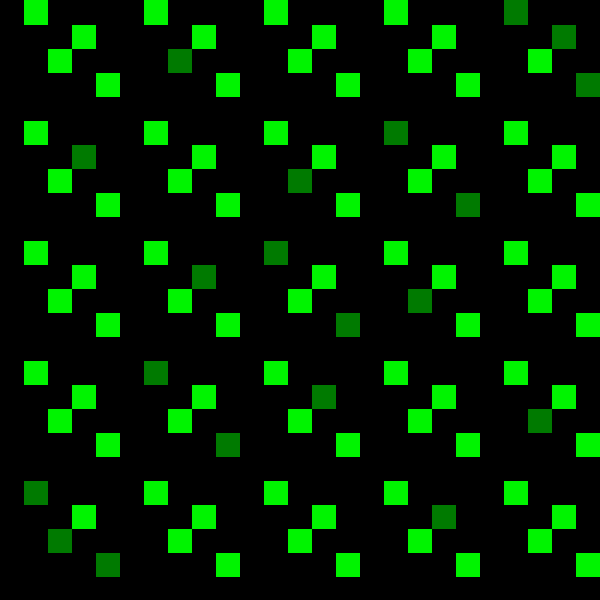
\includegraphics[height=9cm]{iterall_example.png}
				\caption{The dark squares represent systems with lower transient lengths. They seem to exist in each
				direction, though this image only shows two of the four (moving from screen to screen provides the two
				other directions).}
			\end{figure}
			
			As a further reason for exploring this, there are other, more understandable relationships between transient
			lengths of systems when visualised this way; this isn't just a one-off observation. Consider any matrix under 
			a prime-powered modulus where each entry is a multiple of the prime. In this case, the determinant of such a 
			matrix would also be a multiple of the prime, and therefore the matrix would have transient regions since it's 
			not invertible. Now, because this one matrix is not invertible, every other matrix which is "orthogonal" to this 
			matrix (any matrix where only one component is different from the original) will also not be invertible since its
			determinant will necessarily still be a multiple of the prime.
			
			I like to think of these non-invertible matrices as forming rigid spikes which shoot through the module's space.
			They all originate at the zero matrix, then shoot out in all orthogonal directions, branching out whenever we find
			another matrix which satisfies the relation above. In this way, the module essentially has a spiky heart which
			shoots from its center and expands outwards, and a bunch of sparse pockets of transient matrices sprinkled around
			this. The ultimate goal is to better understand how (and why) these matrices are placed the way they are, as well as
			how to better predict the exact transient lengths.
			
			The next section offers a possible way to predict this behaviour, though currently it's been more useful in
			predicting cycle length behaviour as opposed to transient length behaviour.
			
		\ssubsection{Finding Matrices with Non-Increased Cycle Lengths} %ORBITVIS finding darker red squares
			As with transient lengths, the cycle lengths of systems visualised using ORBITVIS' \texttt{iterall} mode also 
			display "oddball" behaviour, though the cycle length case is much easier to explain.
			
			Compared with their corresponding matrices in the prime case, matrices dragged up into a prime-powered modulus
			can either keep their original cycle length, or multiply it by the prime. This can be seen by restricting the
			matrix to its core, then calculating how that matrix must iterate back to the identity matrix mod the prime, then
			extrapolating what it would look like in the prime-powered case (each matrix entry would have an additional 
			$pn$ added to it, which increments regularly whenever the matrix cycles back to the identity mod the prime). 
			
			Because of this behaviour, it's not that surprising to see some matrices retain their original cycle length,
			while others get multiplied by the prime. In fact, when each matrix iterates back to the identity mod the prime,
			their corresponding iterations mod the prime power are fairly predictable in any matrix direction; the $pn$ terms
			tacked on to each component change in a predictable, linear way as you move from matrix to matrix. Using this
			predictability, one can show that, for most matrices in all matrix directions, there must be at least one matrix 
			where the cycle length doesn't increase (which is the rarer behaviour).
			
			More concretely, when you add a multiple of $p^k$ to a single component in a matrix, its behaviour will be
			affected in a linear way, allowing for cycle dynamics to be more easily predicted. To see why, consider an
			arbitrary update matrix $A$ and a matrix $D$ which looks something like
			\[
				D = 
				\begin{bmatrix}
					0 & p^k \\
					0 & 0
				\end{bmatrix}
			\]
	
			If we add $D$ to $A$ and iterate it some number of times, say $\omega$ times, we get
			\[
				(A+D)^{\omega} \equiv A^{\omega} + c_{1}A^{\omega-1}D + d_{1}DA^{\omega-1} + \cdots \mod{p^{k+1}}
			\]
			
			Because matrix multiplication generally isn't commutative, we can't really simplify this expression. However,
			by construction of our matrix $D$, any term with more than one $D$ will equal the zero matrix; multiplying
			twice will force all its terms to have enough powers of the prime to reduce to zero. Therefore, we only need
			to consider those terms with zero or one $D$ factor in them. This is important, as it allows the effect of
			$D$ on $A$ to be linear, in a sense:
			\[
				(A+2D)^{\omega} \equiv A^{\omega} + 2c_{1}A^{\omega-1}D + 2d_{1}DA^{\omega-1} + \cdots \mod{p^{k+1}}
			\]
			
			Multiplying $D$ by any scalar will cause $D$'s effect on $A$'s iteration to be scaled by that scalar. This is
			incredibly useful, as it allows for us to calculate how $A$'s cycle changes when stepping in each orthogonal
			direction, then use that to reason how $A$ changes for a step in \emph{any} direction, since we can linearly 
			combine the different changes to its cycle. This, in turn, allows for a matrix with a non-increased cycle 
			length to be deduced by looking at how $A$ changes.
			
			To see this in action, let's look at a specific example.
			\[
				\begin{bmatrix}
					3 & 3 \\
					4 & 2
				\end{bmatrix}^2 \equiv I \mod{5}
			\]
			so this matrix has a cycle length of 2. Bringing this matrix up to mod 25, we see:
			
			\[
				\begin{bmatrix}
					3 & 3 \\
					4 & 2
				\end{bmatrix}^2 \equiv 
				\begin{bmatrix}
					5(4) + 1 & 5(3) + 0 \\
					5(4) + 0 & 5(3) + 1
				\end{bmatrix} \mod{25}
			\]
			The matrix resembles the identity, though there are these extra bits in each component that reduced
			mod 5, but remain mod 25. Let's see how adding to the matrix's components changes the result.
			
			First, we'll add 5 to the upper-left direction/element:
			\[
				\begin{bmatrix}
					8 & 3 \\
					4 & 2
				\end{bmatrix}^2 \equiv 
				\begin{bmatrix}
					5(0) + 1 & 5(1) + 0 \\
					5(3) + 0 & 5(3) + 1
				\end{bmatrix} \mod{25}
			\]
			Our step in the upper-left matrix direction retained our connection to the identity matrix, yet changed
			the leftover bits.
			
			Now, we'll add 5 to the lower-right direction:
			\[
				\begin{bmatrix}
					3 & 3 \\
					4 & 7
				\end{bmatrix}^2 \equiv
				\begin{bmatrix}
					5(4) + 1 & 5(1) + 0 \\
					5(3) + 0 & 5(2) + 1
				\end{bmatrix} \mod{25}
			\]
			
			Again, we retain our connection to the identity while changing the leftover bits which don't reduce
			mod 25. Can we use these changes to get the matrix to \emph{exactly} the identity?
			
			If we combine one step in the upper-left direction, and three steps in the lower-right direction, we should
			create a matrix which iterates directly to the identity after 2 iterations; the changes caused to the leftover
			bits should reduce all of them to 0:
			\[
				\begin{bmatrix}
					8 & 3 \\
					4 & 17
				\end{bmatrix}^2 \equiv I \mod{25}
			\]
			
			Indeed, this is what we get. By linearly combining the changes caused by orthogonal steps from our original
			matrix, we can find a matrix where the cycle length does not increase when considering a higher modulus.
			
			Quick side note: adding multiples of your prime to matrix directions also affects a matrix's transient region,
			though its connection and utility is a little harder to see and/or utilise. Essentially, the matrix's
			characteristic polynomial will change in a semi-predictable way, eventually creating a polynomial with
			no constant terms. These matrices \emph{tend} to be the oddballs, though for higher-powered moduli the
			connection isn't so straightforward. I don't fully understand the connection myself, so I won't attempt to
			explain it in fear of conveying the wrong idea. It's better to simply play around with ORBITVIS, find these
			"oddball" matrices with different transient lengths, and calculate the characteristic polynomials yourself
			to find the patterns.
			
		\ssubsection{Additive Cycles} %Creating them with matrices; they're NOT 1D cycles
			Eigenvectors in an LCA system can be thought of as being in "one dimensional cycles", since they're locked on
			their own span. Each iteration, they're simply multiplied by some scalar. Because you can have cycles where
			updating a vector is equivalent to multiplying it by a scalar, I got curious as to whether any cycles existed
			where you simply \emph{added} something each iteration. 
			
			The easiest example of an "additive cycle" would be a skew matrix. Using the update matrix $A = 
			\begin{bmatrix}
				\begin{smallmatrix}
					1 & 1 \\
					0 & 1
				\end{smallmatrix}
			\end{bmatrix}
			$ modulo 6, the vector $v = 
			\begin{bmatrix}
				\begin{smallmatrix}
					1 \\
					1
				\end{smallmatrix}
			\end{bmatrix}$ will have the cycle
			\[
				\begin{bmatrix}
					1 \\
					1
				\end{bmatrix}
				\rightarrow
				\begin{bmatrix}
					2 \\
					1
				\end{bmatrix}
				\rightarrow
				\begin{bmatrix}
					3 \\
					1
				\end{bmatrix}
				\rightarrow
				\begin{bmatrix}
					4 \\
					1
				\end{bmatrix}
				\rightarrow
				\begin{bmatrix}
					5 \\
					1
				\end{bmatrix}
				\rightarrow
				\begin{bmatrix}
					0 \\
					1
				\end{bmatrix}
				\rightarrow
				\begin{bmatrix}
					1 \\
					1
				\end{bmatrix}
				\cdots
			\]
			
			To get to the next iteration, we simply add the vector 
			$
				\begin{bmatrix}
					\begin{smallmatrix}
						1 \\
						0
					\end{smallmatrix}
				\end{bmatrix}
			$.
			Creating different types of skew matrices can cause the vector we add each iteration, the "difference vector",
			to change in either of the basis directions. However, I was curious as to whether we can create a matrix with 
			any difference vector we want. In other words, I was curious if we can construct an update matrix such that 
			there's at least one cycle where each new iteration is obtained by adding some arbitrary vector.
			
			The way I attempted to tackle this problem was by framing the addition under some kind of constant difference
			between vector components. Updating a vector by a matrix relies on the components of the vector itself. If the
			components change, so too will the result. If we're dealing with vector cycles greater than 1, then the vector
			itself will change from iteration to iteration. If we want a constant vector to be added to the vector for each
			iteration, we have to keep something about our vector constant, otherwise there's no way matrix multiplication
			could behave the same way for all the different vectors in the cycle. I focused my attention on the difference
			between the components of 2 by 2 vectors, since the components of the vector can still change while keeping the
			difference constant. It also allowed me to focus solely on 2 by 2 systems which kept everything simple.
			
			Now, let's say we wanted to add 
			$
				\begin{bmatrix}
					\begin{smallmatrix}
						5 \\
						4
					\end{smallmatrix}
				\end{bmatrix}
			$
			to our vector each time in order to form our additive cycle. For any vector 
			$
				\begin{bmatrix}
					\begin{smallmatrix}
						x \\
						y
					\end{smallmatrix}
				\end{bmatrix}
			$,
			adding
			$
				\begin{bmatrix}
					\begin{smallmatrix}
						5 \\
						4
					\end{smallmatrix}
				\end{bmatrix}
			$
			to it won't change the value of $4x - 5y$. Therefore, let's set $4x - 5y$ to be our constant difference;
			that's the value we don't want to change within the vectors in our additive cycle.
			
			Now, we'll set $4x - 5y$ to be some arbitrary value. This value will control which vectors we'll have in
			our cycle. For this example, we'll let $4x - 5y \equiv 1$, and we'll make our system modulo 11. Because
			$4x - 5y \equiv 1$, we can say that
			\begin{align*}
				x + 5(4x - 5y) &\equiv x + 5 \\
				y + 4(4x - 5y) &\equiv y + 4
			\end{align*}
			Simplifying the left hand side, we see
			\begin{align*}
				x + 5(4x - 5y) &\equiv x + 20x - 25y &\equiv 21x - 25y &\equiv 10x + 8y &\equiv x + 5 \mod{11} \\
				y + 4(4x - 5y) &\equiv y + 16x - 20y &\equiv 16x - 19y &\equiv  5x + 3y &\equiv y + 4 \mod{11}
			\end{align*}
			So $10x + 8y \equiv x + 5$ and $5x + 3y \equiv y + 4$ in our mod 11 system. Therefore, if we construct 
			the matrix
			\[
				A = 
				\begin{bmatrix}
					10 & 8 \\
					 5 & 3
				\end{bmatrix}
			\]
			then any vector 
			$
				\begin{bmatrix}
					\begin{smallmatrix}
						x \\
						y
					\end{smallmatrix}
				\end{bmatrix}
			$
			where $4x - 5y \equiv 1$ mod 11 will have an additive cycle with difference vector
			$
				\begin{bmatrix}
					\begin{smallmatrix}
						5 \\
						4
					\end{smallmatrix}
				\end{bmatrix}
			$
			under $A$.
			
			As an example, the cycle for the vector 
			$
				\begin{bmatrix}
					\begin{smallmatrix}
						4 \\
						3
					\end{smallmatrix}
				\end{bmatrix}
			$
			under $A$ mod 11 is
			\[
				\begin{bmatrix}
					4 \\
					3
				\end{bmatrix}
				\rightarrow
				\begin{bmatrix}
					9 \\
					7
				\end{bmatrix}
				\rightarrow
				\begin{bmatrix}
					3 \\
					0
				\end{bmatrix}
				\rightarrow
				\begin{bmatrix}
					8 \\
					4
				\end{bmatrix}
				\rightarrow
				\begin{bmatrix}
					2 \\
					8
				\end{bmatrix}
				\rightarrow
				\begin{bmatrix}
					7 \\
					1
				\end{bmatrix}
				\rightarrow
				\begin{bmatrix}
					1 \\
					5
				\end{bmatrix}
				\rightarrow
				\begin{bmatrix}
					6 \\
					9
				\end{bmatrix}
				\rightarrow
				\begin{bmatrix}
					0 \\
					2
				\end{bmatrix}
				\rightarrow
				\begin{bmatrix}
					5 \\
					6
				\end{bmatrix}
				\rightarrow
				\begin{bmatrix}
					10 \\
					10
				\end{bmatrix}
				\rightarrow
				\begin{bmatrix}
					4 \\
					3
				\end{bmatrix}
				\cdots
			\]
			
			To get to the next vector, the vector 
			$
				\begin{bmatrix}
					\begin{smallmatrix}
						5 \\
						4
					\end{smallmatrix}
				\end{bmatrix}
			$
			is added, giving us what I call an "additive cycle".
			
			In general, for any difference vector
			$
				\begin{bmatrix}
					\begin{smallmatrix}
						a \\
						b
					\end{smallmatrix}
				\end{bmatrix}
			$,
			the matrix
			\[
				A = 
				\begin{bmatrix}
					1 + \frac{ab}{c} & \frac{-a^2}{c} \\
					\frac{b^2}{c}    & 1 - \frac{ab}{c}
				\end{bmatrix}
			\]
			will create an additive cycle with the given vector as the difference vector for any vector
			$
				\begin{bmatrix}
					\begin{smallmatrix}
						x \\
						y
					\end{smallmatrix}
				\end{bmatrix}
			$
			where $bx - ay \equiv c$, $c = \text{gcd}(a, b, M)$, $M = $ modulus used.
			
			Given that additive cycles can be created fairly easily for 2 by 2 systems, I'm inclined to wonder how
			such cycles can be created for 3 by 3 systems and higher. I haven't given much thought to such a question,
			though I imagine the process must be fairly similar.
		
	\bibliographystyle{plainnat}
	\bibliography{refs.bib}
	
	\newpage
	We acknowledge the support of the Natural Sciences and Engineering Research Council of Canada (NSERC).

	Nous remercions le Conseil de recherches en sciences naturelles et en génie du Canada (CRSNG) de son soutien.
	
\end{document}
